\documentclass[12pt,a4paper]{article}
\usepackage[abbreviate = true, doi = true, style = nature, giveninits = true, sorting = none, backend = biber]{biblatex}
\usepackage[lmargin = 4cm, rmargin = 4cm, tmargin = 2.5cm, bmargin = 2.5cm]{geometry}
\usepackage[onehalfspacing]{setspace}
\usepackage{graphicx}
\usepackage{hyperref}
\usepackage{times}
\usepackage{csquotes}
\usepackage[UKenglish]{babel}
\usepackage[textsize=tiny]{todonotes}
\usepackage[acronym]{glossaries}
\usepackage{soul} % for command \hl
\usepackage{pdfpages} % to insert pdf docs

\AtBeginBibliography{\small}
\addbibresource{main_sources.bib}

\setlength{\parindent}{0cm}
\setlength{\marginparwidth}{3.5cm} % make todonotes wider
\newcommand{\todoleft}[1]{{\reversemarginpar \todo{#1}}}
% preset for italic species name, abbreviated after first use
\newacronym[first = {\textit{Harmonia axyridis}}]{harm}{\textit{H. axyridis}}{\textit{Harmonia axyridis}}
\glsdisablehyper % no hyperref for \gls


%%%%%%%%%%%%%%%%%%%%%%%%%%%%%%%%%%%%%%%%%%%%%%%%%%%%%%%%%%%%%%%%%%
\begin{document}
\def\findate{\today}

%einreichung-der-bachelorarbeit

\includepdf[pages=-]{deckblatt_einreichung-der-bachelorarbeit.pdf}
%Einverstaendnis mit Veroeffentlichung der Bachelorarbeit
\thispagestyle{empty}
I, Lukas Prader, agree that my bachelor's thesis ("Title"), supervised by Dr. Matthew Talluto, will be digitally archived in a repository of Leopold Franzens University Innsbruck and made available for further academic use. \\

Innsbruck, \findate					\hfill Signature

%title page
\newpage
\thispagestyle{empty}
\begin{center}
    \Large{University of Innsbruck \\ Faculty of Biology} \\
    \vspace{3mm}
    \large{Department of Ecology}
    \vspace{10mm}

    
\includegraphics[width = 0.6 \linewidth]{universitaet-innsbruck-logo-cmyk-farbe.jpg}

    \vspace{10mm}
    \Large{Bachelor Thesis} \\
    \large{submitted for the degree of} \\
    \Large{Bachelor of Science} \\
    \vspace{10mm}
    \LARGE{\textbf{Driving factors in SDM performance through time series: A case study using the invasive species \textit{Harmonia axyridis}}} \\
    \vspace{10mm}

    \large{by \\ Lukas Prader \\ Matriculation Nr.: 12115058 \\ SE Biological Seminar: Ecology}
\end{center}

\vspace{30mm}
\begin{tabular}{ll}
    \large{Submission Date:} & \large{\findate}            \\
    \large{Supervisor:}      & \large{Dr. Matthew Talluto} \\
\end{tabular}

\newpage
\thispagestyle{empty}
\begin{abstract}
    Lorem ipsum
\end{abstract}

\newpage
\tableofcontents
\thispagestyle{empty}
\newpage
\pagenumbering{arabic}

\section{Introduction}
When studying invasive species, it is of particular interest to be able to predict the further development and spread in the invaded range.
The problem of predicting into the unknown is a challenge widespread in the modelling community, and thus an active area of research.
\todo{A bit of jargon you might look up in the SDM literature: ``model transferability''}
\todoleft{If this is the context you want to put your work in, perhaps a little bit more detail here would be useful. Why is this challenging, and in particular for invasive species?}

% Invasion Theory
Invasive species are of special interest in ecological research due to their impact on native ecosystems.
Main goals in this area are to find out which species have potential to become invasive, what habitat will be susceptible to invasion by those species, how fast the species will invade the new area and what impact its invasion will have on the native ecosystem \autocite{shigesada1997invasions}.
To this end, many theories have been created to describe invasion processes.
The invasion of a species can  generally be described with four stages \autocite{blackburn2011invasionstages}:
\begin{enumerate} % just have keywords in a sentence instead of enumeration?
    \item Transport: Leaving the native range, arriving at a new location
    \item Introduction: Existing in specific locations (captivity / cultivation)
    \item Establishment: Existing outside of areas of introduction in the wild
    \item Spread: Sustaining establishment and dispersing to new environments
\end{enumerate}
Depending on the current stage there can be significant differences in behaviour and impact of a species.
The impacts of invasive alien species can be numerous, ranging from food web changes to reductions in habitat and species richness, hydrology and nutrient cycle changes, enhanced invasion of other species and mass extinctions \autocite{simberloff2013invasiveimpacts}.
For example intraguild predation, the predation of species using similar resources, can create completely new stable states of an ecological system \autocite{polis1989theoryIGP}.
Fully understanding the dynamics at play during the invasion process would open more possibilities to actively influence the invasion of threatening species.
For this, creating models which are able to predict the invasion is one current focus of research.
Since invasion theory already uses niche theory, it is quite appropriate to think about applying niche models to the problem.

% SDM Theory
Species Distribution Models (SDMs), are being applied to predict the further development of species occurrences in many contexts, also for invasions.
These types of models have been shown to generate substantial insight into the ecological requirements of species and, as niche models, can be used to predict the potential habitat of a species \autocite{araujo2006sdmchallenges}.
There has been considerable debate on the capabilities and limitations of SDMs, especially when used for prediction outside the data domain.
In general, SDMs are made with the (ideal) assumption that the species is in environmental equilibrium \autocite{elith2009sdmtheory}, implying that its ecological niche is not currently changing.
If these models are now used to predict new, unsampled areas, there actually is no measure to assess their accuracy, since no data is presently available for that area \autocite{araujo2006sdmchallenges}. \todo{more jargon: calibration and validation}
There is also no guarantee that the biotic interactions sampled in the study area will reflect the final interactions in the new area \autocite{elith2009sdmtheory}.
All of these issues apply especially to the prediction of invasive species, since there might be limited data in the invaded range, the species is often not currently at equilibrium and interactions with native species are completely new \autocite{mainali2015sdmprojecting}.
Despite all these challenges, SDMs have been used numerous times to provide insight into the invasive potential and the invasion dynamics of alien species \autocite{zimmermann2010sdmtrends}.
One way of gaining more insight into the invasion process is to create models with data from different time periods during the invasion \autocite{briscoe2019palmerisdm}.
\hl{For example, data from a time period early in the invasion process can be used to build models which then are evaluated against data from a later time period} \autocite{barbet2018nigrithoraxsdm}.
\todoleft{Nice framing thus far. It's just not quite clear to me by this point *why* this is useful. Could you elaborate?}

% Modelling Method
\todoleft{Hmm. This paragraph doesn't really fit here. In fact, maybe this can just go in the methods, as a justification for why you choose ensemble methods.}
\hl{A multitude of Modelling approaches have been developed to model ecological processes.}
In SDMs, methods range from regression methods to machine learning and each feature various strengths and weaknesses, possibly leading to vastly different results for the same dataset.
Due to those differences, a possible approach is to create an ensemble of multiple models \autocite{araujo2007ensemble}.
The way of combining model predictions can vary, but the goal is to improve total performance by combining the results of all computed models.

% Harmonia axyridis
In order to conduct an iterative modelling approach, a species with sufficient data over the time span of invasion is necessary.
\gls{harm}, also known as the Harlequin ladybird or multicoloured Asian lady beetle, is of the family of the Coccinellidae and has its native origin in Asia \autocite{roy2016harmonia}.
At first widely introduced as a control species against pest aphids, \gls{harm} has turned out to be a highly invasive species reaching an almost global distribution \autocite{brown2008harmonia}.
In America, the species was introduced as early as 1916 (California) and in 1988, first populations outside intended release were found \autocite{chapin1991harmoniaNA}.
Usage of \gls{harm} for biological control in Europe dates back as far as 1990 (France) \autocite{coutanceau2006harmoniaFR}.
First invasive occurrences were confirmed in multiple countries during the early 2000s, including Germany (2000), Belgium (2001), the Netherlands (2002) and the United Kingdom (2003) \autocite{roy2016harmonia}.
The first confirmation in Austria, where it was never used for biological control, was in 2006 \autocite{rabitsch2006harmoniaAT}.
% Maybe put vvv in discussion / results to not already spoil the native niche difference.
It has been shown that all established invasive populations outside of North America have their origin in the first established population in eastern North America, with the European populations being significantly influenced by the used biocontrol strain \autocite{lombaert2010harmoniabridgehead}.

The impact of \gls{harm} on invaded areas is diverse.
In some contexts, the ladybird has been shown to have a negative impact on the diversity and abundance of native ladybird species \autocite{roy2016harmonia}.
Many studies show intra guild predation and direct interspecific competition in favour of \gls{harm} \autocite{pell2008harmoniaIGP}.
This results in a large potential for \gls{harm} to be a significant threat for guild diversity and community structure in its introduced ranges.
It has also been shown that the species feeds on a variety of damaged fruit crops, for example grapes, apples, stone fruit and berry crops, making it a pest in these scenarios \autocite{koch2004harmoniafoodcrop}.
The aggregating behaviour of \gls{harm}, mostly as a strategy for overwintering, is also a cause of disturbance, since private homes and facilities are invaded by large amounts of beetles at a given time \autocite{nalepa2005harmoniahomes}.
In general, \gls{harm} can be concluded to be a species with high impact as an invader, and thus of interest for active research questions.
\todoleft{I think this is a fine introduction to the species. But you start in the previous paragraph by stating that you need a species with sufficient data. Is this the case? It might be obvious, but you never state so.}

%existing SDMs for H. axyridis
There have been several publications which model and predict the distribution of \gls{harm}, constrained to certain geographical ranges (i.e. Spain \autocite{ameixa2019harmSDMSpain}, Chile \autocite{alaniz2018harmSDMChile}) or even on global scales \autocite{bidinger2012harmSDMglobalMaxent, poutsma2008harmSDMglobalClimex}.
There has not yet been any model iteration in form of a time series, which is what this thesis aims to add as new insight.
Another goal of this thesis is to look into the limitations of models built early in the invasion process of a species.
By iterating over the years of the invasion, model performance can be evaluated with consideration to the current state of invasion.
In the end, a better understanding of the invasion process of \gls{harm} in Europe and the performance of models trying to capture it should be the result.



\newpage
\section{Materials and Methods}
This section elaborates on the Methods used to conduct this research.

\subsection{Datasets}
For occurrence data, all global occurrences of \gls{harm} were downloaded from the GBIF database \autocite{GBIFaxyridisdataset}.
All traditional 19 bioclim variables were obtained from the CHELSA V2.1 climatologies dataset \autocite{karger2017CHELSApaper, CHELSAbioclimdataset}, using the 1981-2010 time frame for all years from 2002 to 2010 as well as the MPI-ESM 1.2 ssp370 scenario 2011-2040 for all years from 2011 to 2022.
As additional information, land cover data was used from the Copernicus Land cover Classification dataset \autocite{COPlandcoverdataset}  with yearly resolution for 2002 up to 2020.

\subsection{Data preparation}
All bioclim and land cover layers were resampled to a matching resolution of 30 arc seconds and cropped to two spatial extents, Europe and the presumed native range referencing (Orlova-Bienkowskaja, Ukrainsky \& Brown, 2015) \autocite{orlova2015harmonia}.

The presence-only points from GBIF were checked for missing values for latitude, longitude, year or coordinate uncertainty and then subset to the afore mentioned spatial extents.
No occurrences after 2022 were used, also no points with a coordinate uncertainty larger than 1 km.
In Europe, the initial cut off year for presences was 1991, since this is the year of invasion according to the EASIN website.
Afterwards, using the library \texttt{CoordinateCleaner}, all remaining data points were again checked for common errors or biases in the respective subset (tests used: "capitals", "centroids", "duplicates", "equal", "institutions", "outliers", "seas", "zeros").
In addition, all occurrences were checked for their land cover class values in their respective year, removing points in the water or with no data.
In the end, remaining data points prior to 2002 were deemed insignificant and removed from the dataset.
To prepare the data for modelling, pseudoabsences were generated for each year, randomly sampling the area and resampling points in the water or with no data.

To correct for sampling bias in the data, the European extent was split into sub extents in order to add additional absences to denser sampled regions.
For this, an algorithm was written which splits a given extent in half and continues to do so with the created sub-extents until the amount of points in the extents is at most some chosen number.
For the first part of absence generation completely random absences are drawn from the original extent in order to ensure at least some coverage of the whole study area.
In the second step, additional absences are generated for each subextent separately and in relation to the amount of presences inside the respective subextent.
This results in more absences in regions with more presences as well (visual representation in figure \ref{fig:ext_subdiv} A).
The subdivision of the dataset was carried out using all presences in Europe over all years and setting the threshold to be $\leq$ 30\%, leading to sub-extents converging around the United Kingdom and the Netherlands, which seem to have been sampled very intensely (fig. \ref{fig:ext_subdiv} B).
For the first and second step of absence generation, absences equal to and twice the amount of presences were generated respectively, resulting in three absences per presence in total.

\begin{figure}[!h]
    \centering
    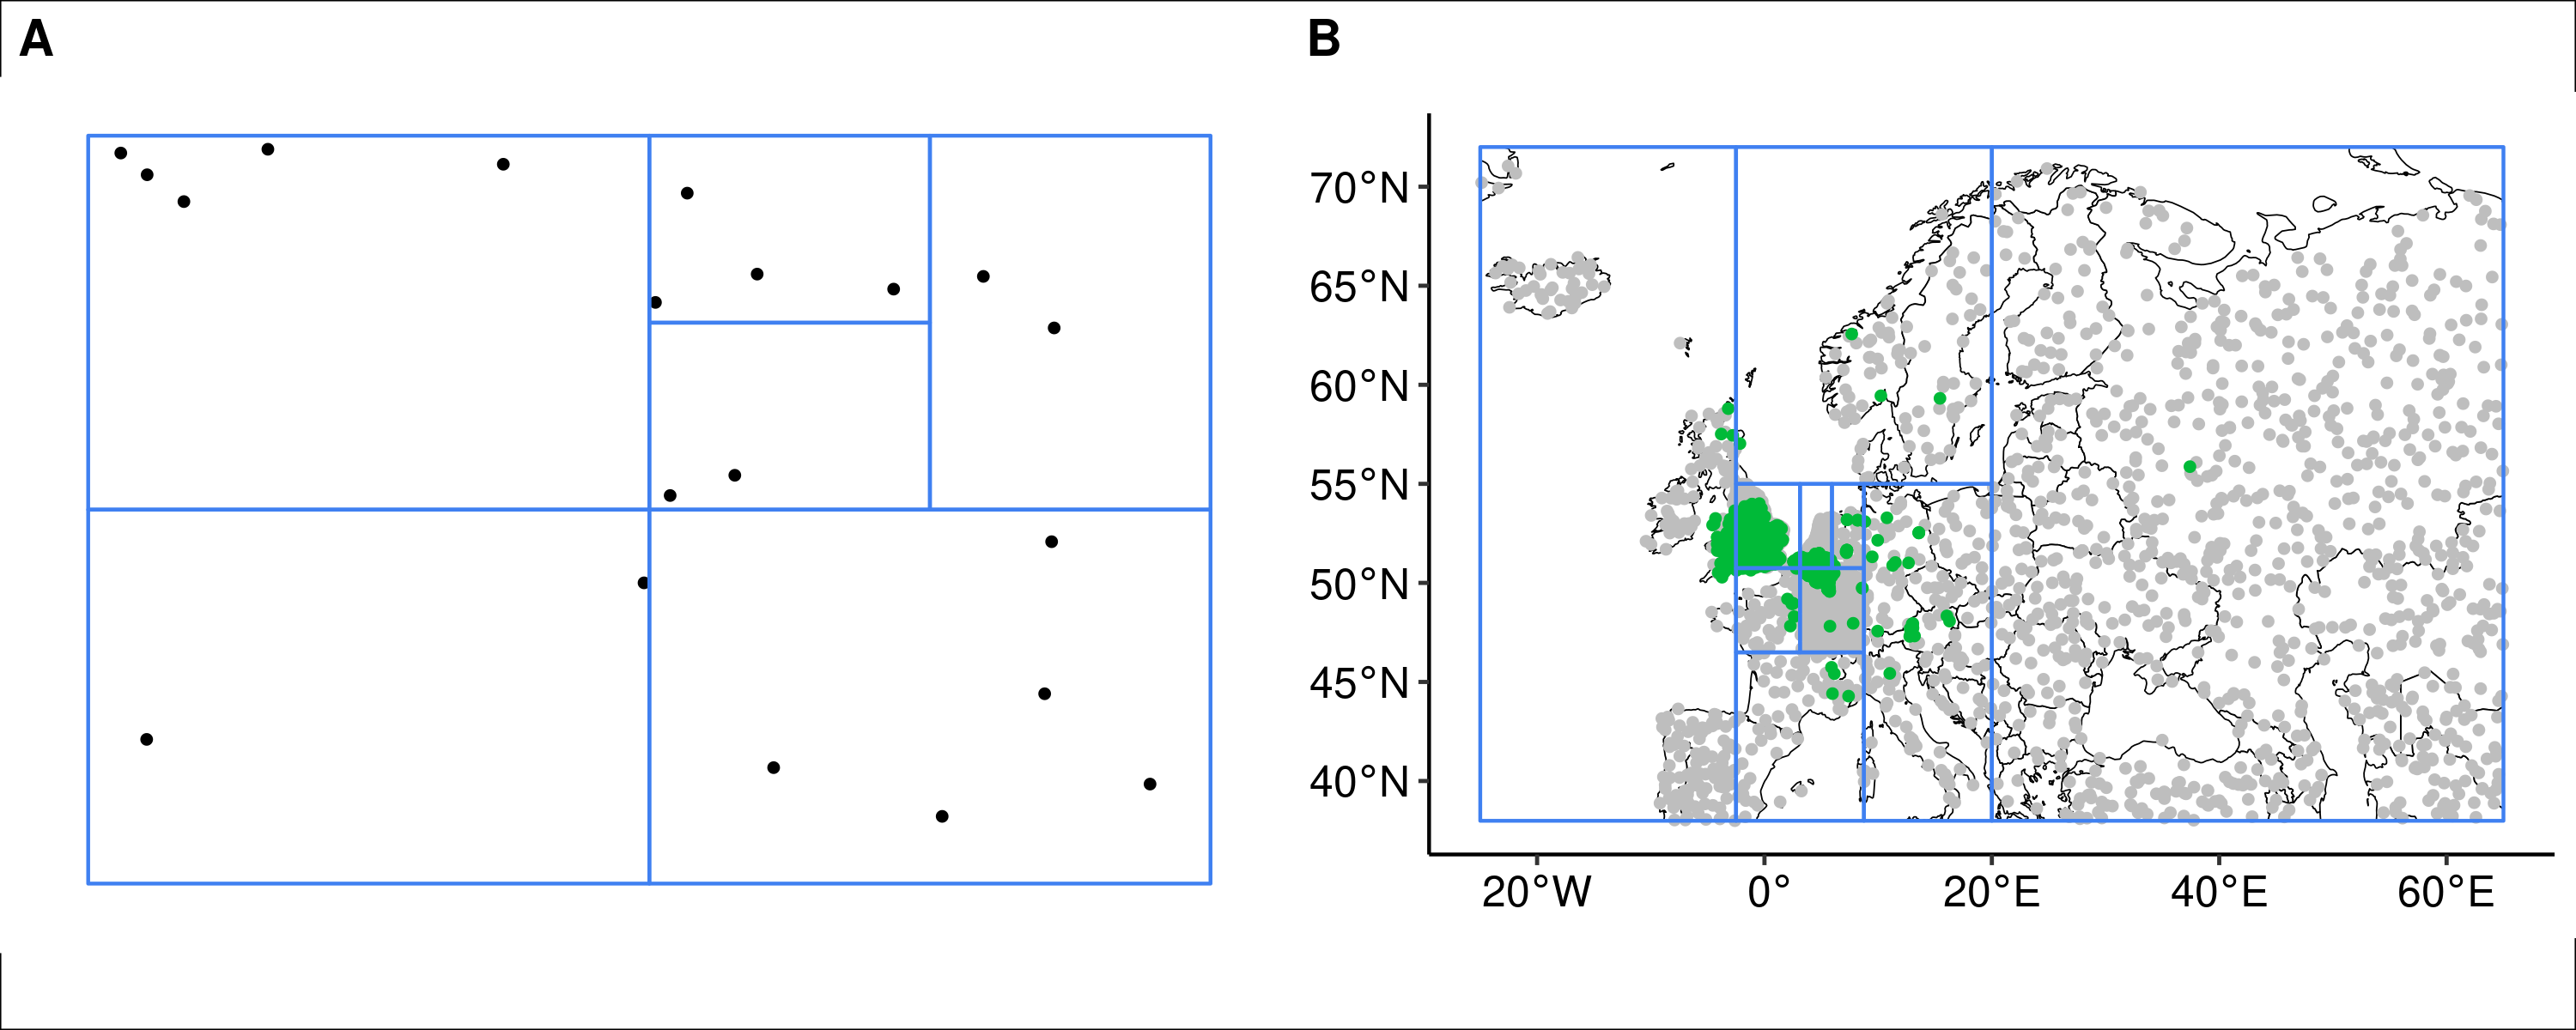
\includegraphics[width = 0.8\linewidth]{"../../R/figures/ext-subdiv.png"}
    \caption{\label{fig:ext_subdiv} Visualization of the subdivision algorithm and absence generation. Subfigure A shows an example of 30 generated presences(green), subdivided with a threshold of $\leq$ 10 points per subextent. The generated absences are shown in black, with circles indicating the first 30 completely random absences, and asterisks indicating absences generated relative to the amount of presences in a subextent. Subfigure B shows the calculated subextents for the total presences of the dataset, with presences(green) and absences(grey) for 2008 plotted as an example.}
\end{figure}

\subsection{Model building}
For each year, the following Models were computed: General Linear (GLM) \autocite{guisan2002glm-gam}, General Additive (GAM) \autocite{guisan2002glm-gam}, Boosted Regression Trees (BRT) \autocite{elith2008brt} and Maximum Entropy (MAXENT) \autocite{phillips2017maxnet}.
A model for a specific year always included all points from past years as well.
The iterative models that were built only use data points from Europe, though there was one model created only with native occurrences and predicted for each year in Europe.
For all used occurrence points after 2020, the land cover data of 2020 was used as a substitute.

Variance inflation factors were used to select the variables used for model building.
For this, a GAM was computed only using Europe data from 2002, using all bioclim and land cover variables.
For land cover variables, a PCA was computed on the relative area of all land cover classes in an 18 km radius around 5000 random data points in Europe, subsequently projecting the occurrence data onto the resulting axes.
The 18 km radius was chosen, since it is the average flight distance determined for \gls{harm} \autocite{jeffries2013flightharmonia}.
PCA axes were included in the model until a cut-off of 80\% of explained variance was reached.
Variance inflation factors were computed for this GAM and the variable with the highest VIF was dropped until none of the remaining variables had a VIF greater than 10.

\subsection{Analysis}
All SDM models of each year were evaluated for their accuracy on predicting the occurrences of the following year and the final year of 2022 using the True Skill Statistic (TSS).
The TSS values were used to create a TSS-weighted ensemble of all model predictions, which was again evaluated for its accuracy.
For each year, the occupied niche was computed by running a PCA analysis on the bioclim variables.
The niche was then visualized by plotting a dynamic occurrence density grid for the first two PCA axes \autocite{broennimann2012niche}.
The overlap between each year for Europe and the respective following year was computed, as well as a niche similarity and niche equivalency test.
Niche overlap for the total EU data was also visualized in comparison to the total native niche.
All mentioned niche analyses were conducted using the library \texttt{ecospat} \autocite{dicola2017ecospat}.
The development of TSS over time was tested for correlation with the amount of training data and the niche overlap for a given year, using the pearson correlation test.

\newpage

\section{Results}

\section{Discussion}

\section{Conclusion}

\section{Acknowledgements}


\newpage
\printbibliography[]
\newpage
\appendix
Appendix

\end{document}